\documentclass[11pt]{article}

    \usepackage[breakable]{tcolorbox}
    \usepackage{parskip} % Stop auto-indenting (to mimic markdown behaviour)
    
    \usepackage{iftex}
    \ifPDFTeX
    	\usepackage[T1]{fontenc}
    	\usepackage{mathpazo}
    \else
    	\usepackage{fontspec}
    \fi

    % Basic figure setup, for now with no caption control since it's done
    % automatically by Pandoc (which extracts ![](path) syntax from Markdown).
    \usepackage{graphicx}
    % Maintain compatibility with old templates. Remove in nbconvert 6.0
    \let\Oldincludegraphics\includegraphics
    % Ensure that by default, figures have no caption (until we provide a
    % proper Figure object with a Caption API and a way to capture that
    % in the conversion process - todo).
    \usepackage{caption}
    \DeclareCaptionFormat{nocaption}{}
    \captionsetup{format=nocaption,aboveskip=0pt,belowskip=0pt}

    \usepackage{float}
    \floatplacement{figure}{H} % forces figures to be placed at the correct location
    \usepackage{xcolor} % Allow colors to be defined
    \usepackage{enumerate} % Needed for markdown enumerations to work
    \usepackage{geometry} % Used to adjust the document margins
    \usepackage{amsmath} % Equations
    \usepackage{amssymb} % Equations
    \usepackage{textcomp} % defines textquotesingle
    % Hack from http://tex.stackexchange.com/a/47451/13684:
    \AtBeginDocument{%
        \def\PYZsq{\textquotesingle}% Upright quotes in Pygmentized code
    }
    \usepackage{upquote} % Upright quotes for verbatim code
    \usepackage{eurosym} % defines \euro
    \usepackage[mathletters]{ucs} % Extended unicode (utf-8) support
    \usepackage{fancyvrb} % verbatim replacement that allows latex
    \usepackage{grffile} % extends the file name processing of package graphics 
                         % to support a larger range
    \makeatletter % fix for old versions of grffile with XeLaTeX
    \@ifpackagelater{grffile}{2019/11/01}
    {
      % Do nothing on new versions
    }
    {
      \def\Gread@@xetex#1{%
        \IfFileExists{"\Gin@base".bb}%
        {\Gread@eps{\Gin@base.bb}}%
        {\Gread@@xetex@aux#1}%
      }
    }
    \makeatother
    \usepackage[Export]{adjustbox} % Used to constrain images to a maximum size
    \adjustboxset{max size={0.9\linewidth}{0.9\paperheight}}

    % The hyperref package gives us a pdf with properly built
    % internal navigation ('pdf bookmarks' for the table of contents,
    % internal cross-reference links, web links for URLs, etc.)
    \usepackage{hyperref}
    % The default LaTeX title has an obnoxious amount of whitespace. By default,
    % titling removes some of it. It also provides customization options.
    \usepackage{titling}
    \usepackage{longtable} % longtable support required by pandoc >1.10
    \usepackage{booktabs}  % table support for pandoc > 1.12.2
    \usepackage[inline]{enumitem} % IRkernel/repr support (it uses the enumerate* environment)
    \usepackage[normalem]{ulem} % ulem is needed to support strikethroughs (\sout)
                                % normalem makes italics be italics, not underlines
    \usepackage{mathrsfs}
    

    
    % Colors for the hyperref package
    \definecolor{urlcolor}{rgb}{0,.145,.698}
    \definecolor{linkcolor}{rgb}{.71,0.21,0.01}
    \definecolor{citecolor}{rgb}{.12,.54,.11}

    % ANSI colors
    \definecolor{ansi-black}{HTML}{3E424D}
    \definecolor{ansi-black-intense}{HTML}{282C36}
    \definecolor{ansi-red}{HTML}{E75C58}
    \definecolor{ansi-red-intense}{HTML}{B22B31}
    \definecolor{ansi-green}{HTML}{00A250}
    \definecolor{ansi-green-intense}{HTML}{007427}
    \definecolor{ansi-yellow}{HTML}{DDB62B}
    \definecolor{ansi-yellow-intense}{HTML}{B27D12}
    \definecolor{ansi-blue}{HTML}{208FFB}
    \definecolor{ansi-blue-intense}{HTML}{0065CA}
    \definecolor{ansi-magenta}{HTML}{D160C4}
    \definecolor{ansi-magenta-intense}{HTML}{A03196}
    \definecolor{ansi-cyan}{HTML}{60C6C8}
    \definecolor{ansi-cyan-intense}{HTML}{258F8F}
    \definecolor{ansi-white}{HTML}{C5C1B4}
    \definecolor{ansi-white-intense}{HTML}{A1A6B2}
    \definecolor{ansi-default-inverse-fg}{HTML}{FFFFFF}
    \definecolor{ansi-default-inverse-bg}{HTML}{000000}

    % common color for the border for error outputs.
    \definecolor{outerrorbackground}{HTML}{FFDFDF}

    % commands and environments needed by pandoc snippets
    % extracted from the output of `pandoc -s`
    \providecommand{\tightlist}{%
      \setlength{\itemsep}{0pt}\setlength{\parskip}{0pt}}
    \DefineVerbatimEnvironment{Highlighting}{Verbatim}{commandchars=\\\{\}}
    % Add ',fontsize=\small' for more characters per line
    \newenvironment{Shaded}{}{}
    \newcommand{\KeywordTok}[1]{\textcolor[rgb]{0.00,0.44,0.13}{\textbf{{#1}}}}
    \newcommand{\DataTypeTok}[1]{\textcolor[rgb]{0.56,0.13,0.00}{{#1}}}
    \newcommand{\DecValTok}[1]{\textcolor[rgb]{0.25,0.63,0.44}{{#1}}}
    \newcommand{\BaseNTok}[1]{\textcolor[rgb]{0.25,0.63,0.44}{{#1}}}
    \newcommand{\FloatTok}[1]{\textcolor[rgb]{0.25,0.63,0.44}{{#1}}}
    \newcommand{\CharTok}[1]{\textcolor[rgb]{0.25,0.44,0.63}{{#1}}}
    \newcommand{\StringTok}[1]{\textcolor[rgb]{0.25,0.44,0.63}{{#1}}}
    \newcommand{\CommentTok}[1]{\textcolor[rgb]{0.38,0.63,0.69}{\textit{{#1}}}}
    \newcommand{\OtherTok}[1]{\textcolor[rgb]{0.00,0.44,0.13}{{#1}}}
    \newcommand{\AlertTok}[1]{\textcolor[rgb]{1.00,0.00,0.00}{\textbf{{#1}}}}
    \newcommand{\FunctionTok}[1]{\textcolor[rgb]{0.02,0.16,0.49}{{#1}}}
    \newcommand{\RegionMarkerTok}[1]{{#1}}
    \newcommand{\ErrorTok}[1]{\textcolor[rgb]{1.00,0.00,0.00}{\textbf{{#1}}}}
    \newcommand{\NormalTok}[1]{{#1}}
    
    % Additional commands for more recent versions of Pandoc
    \newcommand{\ConstantTok}[1]{\textcolor[rgb]{0.53,0.00,0.00}{{#1}}}
    \newcommand{\SpecialCharTok}[1]{\textcolor[rgb]{0.25,0.44,0.63}{{#1}}}
    \newcommand{\VerbatimStringTok}[1]{\textcolor[rgb]{0.25,0.44,0.63}{{#1}}}
    \newcommand{\SpecialStringTok}[1]{\textcolor[rgb]{0.73,0.40,0.53}{{#1}}}
    \newcommand{\ImportTok}[1]{{#1}}
    \newcommand{\DocumentationTok}[1]{\textcolor[rgb]{0.73,0.13,0.13}{\textit{{#1}}}}
    \newcommand{\AnnotationTok}[1]{\textcolor[rgb]{0.38,0.63,0.69}{\textbf{\textit{{#1}}}}}
    \newcommand{\CommentVarTok}[1]{\textcolor[rgb]{0.38,0.63,0.69}{\textbf{\textit{{#1}}}}}
    \newcommand{\VariableTok}[1]{\textcolor[rgb]{0.10,0.09,0.49}{{#1}}}
    \newcommand{\ControlFlowTok}[1]{\textcolor[rgb]{0.00,0.44,0.13}{\textbf{{#1}}}}
    \newcommand{\OperatorTok}[1]{\textcolor[rgb]{0.40,0.40,0.40}{{#1}}}
    \newcommand{\BuiltInTok}[1]{{#1}}
    \newcommand{\ExtensionTok}[1]{{#1}}
    \newcommand{\PreprocessorTok}[1]{\textcolor[rgb]{0.74,0.48,0.00}{{#1}}}
    \newcommand{\AttributeTok}[1]{\textcolor[rgb]{0.49,0.56,0.16}{{#1}}}
    \newcommand{\InformationTok}[1]{\textcolor[rgb]{0.38,0.63,0.69}{\textbf{\textit{{#1}}}}}
    \newcommand{\WarningTok}[1]{\textcolor[rgb]{0.38,0.63,0.69}{\textbf{\textit{{#1}}}}}
    
    
    % Define a nice break command that doesn't care if a line doesn't already
    % exist.
    \def\br{\hspace*{\fill} \\* }
    % Math Jax compatibility definitions
    \def\gt{>}
    \def\lt{<}
    \let\Oldtex\TeX
    \let\Oldlatex\LaTeX
    \renewcommand{\TeX}{\textrm{\Oldtex}}
    \renewcommand{\LaTeX}{\textrm{\Oldlatex}}
    % Document parameters
    % Document title
    \title{3.3 Odometry-based motion model}
    
    
    
    
    
% Pygments definitions
\makeatletter
\def\PY@reset{\let\PY@it=\relax \let\PY@bf=\relax%
    \let\PY@ul=\relax \let\PY@tc=\relax%
    \let\PY@bc=\relax \let\PY@ff=\relax}
\def\PY@tok#1{\csname PY@tok@#1\endcsname}
\def\PY@toks#1+{\ifx\relax#1\empty\else%
    \PY@tok{#1}\expandafter\PY@toks\fi}
\def\PY@do#1{\PY@bc{\PY@tc{\PY@ul{%
    \PY@it{\PY@bf{\PY@ff{#1}}}}}}}
\def\PY#1#2{\PY@reset\PY@toks#1+\relax+\PY@do{#2}}

\expandafter\def\csname PY@tok@w\endcsname{\def\PY@tc##1{\textcolor[rgb]{0.73,0.73,0.73}{##1}}}
\expandafter\def\csname PY@tok@c\endcsname{\let\PY@it=\textit\def\PY@tc##1{\textcolor[rgb]{0.25,0.50,0.50}{##1}}}
\expandafter\def\csname PY@tok@cp\endcsname{\def\PY@tc##1{\textcolor[rgb]{0.74,0.48,0.00}{##1}}}
\expandafter\def\csname PY@tok@k\endcsname{\let\PY@bf=\textbf\def\PY@tc##1{\textcolor[rgb]{0.00,0.50,0.00}{##1}}}
\expandafter\def\csname PY@tok@kp\endcsname{\def\PY@tc##1{\textcolor[rgb]{0.00,0.50,0.00}{##1}}}
\expandafter\def\csname PY@tok@kt\endcsname{\def\PY@tc##1{\textcolor[rgb]{0.69,0.00,0.25}{##1}}}
\expandafter\def\csname PY@tok@o\endcsname{\def\PY@tc##1{\textcolor[rgb]{0.40,0.40,0.40}{##1}}}
\expandafter\def\csname PY@tok@ow\endcsname{\let\PY@bf=\textbf\def\PY@tc##1{\textcolor[rgb]{0.67,0.13,1.00}{##1}}}
\expandafter\def\csname PY@tok@nb\endcsname{\def\PY@tc##1{\textcolor[rgb]{0.00,0.50,0.00}{##1}}}
\expandafter\def\csname PY@tok@nf\endcsname{\def\PY@tc##1{\textcolor[rgb]{0.00,0.00,1.00}{##1}}}
\expandafter\def\csname PY@tok@nc\endcsname{\let\PY@bf=\textbf\def\PY@tc##1{\textcolor[rgb]{0.00,0.00,1.00}{##1}}}
\expandafter\def\csname PY@tok@nn\endcsname{\let\PY@bf=\textbf\def\PY@tc##1{\textcolor[rgb]{0.00,0.00,1.00}{##1}}}
\expandafter\def\csname PY@tok@ne\endcsname{\let\PY@bf=\textbf\def\PY@tc##1{\textcolor[rgb]{0.82,0.25,0.23}{##1}}}
\expandafter\def\csname PY@tok@nv\endcsname{\def\PY@tc##1{\textcolor[rgb]{0.10,0.09,0.49}{##1}}}
\expandafter\def\csname PY@tok@no\endcsname{\def\PY@tc##1{\textcolor[rgb]{0.53,0.00,0.00}{##1}}}
\expandafter\def\csname PY@tok@nl\endcsname{\def\PY@tc##1{\textcolor[rgb]{0.63,0.63,0.00}{##1}}}
\expandafter\def\csname PY@tok@ni\endcsname{\let\PY@bf=\textbf\def\PY@tc##1{\textcolor[rgb]{0.60,0.60,0.60}{##1}}}
\expandafter\def\csname PY@tok@na\endcsname{\def\PY@tc##1{\textcolor[rgb]{0.49,0.56,0.16}{##1}}}
\expandafter\def\csname PY@tok@nt\endcsname{\let\PY@bf=\textbf\def\PY@tc##1{\textcolor[rgb]{0.00,0.50,0.00}{##1}}}
\expandafter\def\csname PY@tok@nd\endcsname{\def\PY@tc##1{\textcolor[rgb]{0.67,0.13,1.00}{##1}}}
\expandafter\def\csname PY@tok@s\endcsname{\def\PY@tc##1{\textcolor[rgb]{0.73,0.13,0.13}{##1}}}
\expandafter\def\csname PY@tok@sd\endcsname{\let\PY@it=\textit\def\PY@tc##1{\textcolor[rgb]{0.73,0.13,0.13}{##1}}}
\expandafter\def\csname PY@tok@si\endcsname{\let\PY@bf=\textbf\def\PY@tc##1{\textcolor[rgb]{0.73,0.40,0.53}{##1}}}
\expandafter\def\csname PY@tok@se\endcsname{\let\PY@bf=\textbf\def\PY@tc##1{\textcolor[rgb]{0.73,0.40,0.13}{##1}}}
\expandafter\def\csname PY@tok@sr\endcsname{\def\PY@tc##1{\textcolor[rgb]{0.73,0.40,0.53}{##1}}}
\expandafter\def\csname PY@tok@ss\endcsname{\def\PY@tc##1{\textcolor[rgb]{0.10,0.09,0.49}{##1}}}
\expandafter\def\csname PY@tok@sx\endcsname{\def\PY@tc##1{\textcolor[rgb]{0.00,0.50,0.00}{##1}}}
\expandafter\def\csname PY@tok@m\endcsname{\def\PY@tc##1{\textcolor[rgb]{0.40,0.40,0.40}{##1}}}
\expandafter\def\csname PY@tok@gh\endcsname{\let\PY@bf=\textbf\def\PY@tc##1{\textcolor[rgb]{0.00,0.00,0.50}{##1}}}
\expandafter\def\csname PY@tok@gu\endcsname{\let\PY@bf=\textbf\def\PY@tc##1{\textcolor[rgb]{0.50,0.00,0.50}{##1}}}
\expandafter\def\csname PY@tok@gd\endcsname{\def\PY@tc##1{\textcolor[rgb]{0.63,0.00,0.00}{##1}}}
\expandafter\def\csname PY@tok@gi\endcsname{\def\PY@tc##1{\textcolor[rgb]{0.00,0.63,0.00}{##1}}}
\expandafter\def\csname PY@tok@gr\endcsname{\def\PY@tc##1{\textcolor[rgb]{1.00,0.00,0.00}{##1}}}
\expandafter\def\csname PY@tok@ge\endcsname{\let\PY@it=\textit}
\expandafter\def\csname PY@tok@gs\endcsname{\let\PY@bf=\textbf}
\expandafter\def\csname PY@tok@gp\endcsname{\let\PY@bf=\textbf\def\PY@tc##1{\textcolor[rgb]{0.00,0.00,0.50}{##1}}}
\expandafter\def\csname PY@tok@go\endcsname{\def\PY@tc##1{\textcolor[rgb]{0.53,0.53,0.53}{##1}}}
\expandafter\def\csname PY@tok@gt\endcsname{\def\PY@tc##1{\textcolor[rgb]{0.00,0.27,0.87}{##1}}}
\expandafter\def\csname PY@tok@err\endcsname{\def\PY@bc##1{\setlength{\fboxsep}{0pt}\fcolorbox[rgb]{1.00,0.00,0.00}{1,1,1}{\strut ##1}}}
\expandafter\def\csname PY@tok@kc\endcsname{\let\PY@bf=\textbf\def\PY@tc##1{\textcolor[rgb]{0.00,0.50,0.00}{##1}}}
\expandafter\def\csname PY@tok@kd\endcsname{\let\PY@bf=\textbf\def\PY@tc##1{\textcolor[rgb]{0.00,0.50,0.00}{##1}}}
\expandafter\def\csname PY@tok@kn\endcsname{\let\PY@bf=\textbf\def\PY@tc##1{\textcolor[rgb]{0.00,0.50,0.00}{##1}}}
\expandafter\def\csname PY@tok@kr\endcsname{\let\PY@bf=\textbf\def\PY@tc##1{\textcolor[rgb]{0.00,0.50,0.00}{##1}}}
\expandafter\def\csname PY@tok@bp\endcsname{\def\PY@tc##1{\textcolor[rgb]{0.00,0.50,0.00}{##1}}}
\expandafter\def\csname PY@tok@fm\endcsname{\def\PY@tc##1{\textcolor[rgb]{0.00,0.00,1.00}{##1}}}
\expandafter\def\csname PY@tok@vc\endcsname{\def\PY@tc##1{\textcolor[rgb]{0.10,0.09,0.49}{##1}}}
\expandafter\def\csname PY@tok@vg\endcsname{\def\PY@tc##1{\textcolor[rgb]{0.10,0.09,0.49}{##1}}}
\expandafter\def\csname PY@tok@vi\endcsname{\def\PY@tc##1{\textcolor[rgb]{0.10,0.09,0.49}{##1}}}
\expandafter\def\csname PY@tok@vm\endcsname{\def\PY@tc##1{\textcolor[rgb]{0.10,0.09,0.49}{##1}}}
\expandafter\def\csname PY@tok@sa\endcsname{\def\PY@tc##1{\textcolor[rgb]{0.73,0.13,0.13}{##1}}}
\expandafter\def\csname PY@tok@sb\endcsname{\def\PY@tc##1{\textcolor[rgb]{0.73,0.13,0.13}{##1}}}
\expandafter\def\csname PY@tok@sc\endcsname{\def\PY@tc##1{\textcolor[rgb]{0.73,0.13,0.13}{##1}}}
\expandafter\def\csname PY@tok@dl\endcsname{\def\PY@tc##1{\textcolor[rgb]{0.73,0.13,0.13}{##1}}}
\expandafter\def\csname PY@tok@s2\endcsname{\def\PY@tc##1{\textcolor[rgb]{0.73,0.13,0.13}{##1}}}
\expandafter\def\csname PY@tok@sh\endcsname{\def\PY@tc##1{\textcolor[rgb]{0.73,0.13,0.13}{##1}}}
\expandafter\def\csname PY@tok@s1\endcsname{\def\PY@tc##1{\textcolor[rgb]{0.73,0.13,0.13}{##1}}}
\expandafter\def\csname PY@tok@mb\endcsname{\def\PY@tc##1{\textcolor[rgb]{0.40,0.40,0.40}{##1}}}
\expandafter\def\csname PY@tok@mf\endcsname{\def\PY@tc##1{\textcolor[rgb]{0.40,0.40,0.40}{##1}}}
\expandafter\def\csname PY@tok@mh\endcsname{\def\PY@tc##1{\textcolor[rgb]{0.40,0.40,0.40}{##1}}}
\expandafter\def\csname PY@tok@mi\endcsname{\def\PY@tc##1{\textcolor[rgb]{0.40,0.40,0.40}{##1}}}
\expandafter\def\csname PY@tok@il\endcsname{\def\PY@tc##1{\textcolor[rgb]{0.40,0.40,0.40}{##1}}}
\expandafter\def\csname PY@tok@mo\endcsname{\def\PY@tc##1{\textcolor[rgb]{0.40,0.40,0.40}{##1}}}
\expandafter\def\csname PY@tok@ch\endcsname{\let\PY@it=\textit\def\PY@tc##1{\textcolor[rgb]{0.25,0.50,0.50}{##1}}}
\expandafter\def\csname PY@tok@cm\endcsname{\let\PY@it=\textit\def\PY@tc##1{\textcolor[rgb]{0.25,0.50,0.50}{##1}}}
\expandafter\def\csname PY@tok@cpf\endcsname{\let\PY@it=\textit\def\PY@tc##1{\textcolor[rgb]{0.25,0.50,0.50}{##1}}}
\expandafter\def\csname PY@tok@c1\endcsname{\let\PY@it=\textit\def\PY@tc##1{\textcolor[rgb]{0.25,0.50,0.50}{##1}}}
\expandafter\def\csname PY@tok@cs\endcsname{\let\PY@it=\textit\def\PY@tc##1{\textcolor[rgb]{0.25,0.50,0.50}{##1}}}

\def\PYZbs{\char`\\}
\def\PYZus{\char`\_}
\def\PYZob{\char`\{}
\def\PYZcb{\char`\}}
\def\PYZca{\char`\^}
\def\PYZam{\char`\&}
\def\PYZlt{\char`\<}
\def\PYZgt{\char`\>}
\def\PYZsh{\char`\#}
\def\PYZpc{\char`\%}
\def\PYZdl{\char`\$}
\def\PYZhy{\char`\-}
\def\PYZsq{\char`\'}
\def\PYZdq{\char`\"}
\def\PYZti{\char`\~}
% for compatibility with earlier versions
\def\PYZat{@}
\def\PYZlb{[}
\def\PYZrb{]}
\makeatother


    % For linebreaks inside Verbatim environment from package fancyvrb. 
    \makeatletter
        \newbox\Wrappedcontinuationbox 
        \newbox\Wrappedvisiblespacebox 
        \newcommand*\Wrappedvisiblespace {\textcolor{red}{\textvisiblespace}} 
        \newcommand*\Wrappedcontinuationsymbol {\textcolor{red}{\llap{\tiny$\m@th\hookrightarrow$}}} 
        \newcommand*\Wrappedcontinuationindent {3ex } 
        \newcommand*\Wrappedafterbreak {\kern\Wrappedcontinuationindent\copy\Wrappedcontinuationbox} 
        % Take advantage of the already applied Pygments mark-up to insert 
        % potential linebreaks for TeX processing. 
        %        {, <, #, %, $, ' and ": go to next line. 
        %        _, }, ^, &, >, - and ~: stay at end of broken line. 
        % Use of \textquotesingle for straight quote. 
        \newcommand*\Wrappedbreaksatspecials {% 
            \def\PYGZus{\discretionary{\char`\_}{\Wrappedafterbreak}{\char`\_}}% 
            \def\PYGZob{\discretionary{}{\Wrappedafterbreak\char`\{}{\char`\{}}% 
            \def\PYGZcb{\discretionary{\char`\}}{\Wrappedafterbreak}{\char`\}}}% 
            \def\PYGZca{\discretionary{\char`\^}{\Wrappedafterbreak}{\char`\^}}% 
            \def\PYGZam{\discretionary{\char`\&}{\Wrappedafterbreak}{\char`\&}}% 
            \def\PYGZlt{\discretionary{}{\Wrappedafterbreak\char`\<}{\char`\<}}% 
            \def\PYGZgt{\discretionary{\char`\>}{\Wrappedafterbreak}{\char`\>}}% 
            \def\PYGZsh{\discretionary{}{\Wrappedafterbreak\char`\#}{\char`\#}}% 
            \def\PYGZpc{\discretionary{}{\Wrappedafterbreak\char`\%}{\char`\%}}% 
            \def\PYGZdl{\discretionary{}{\Wrappedafterbreak\char`\$}{\char`\$}}% 
            \def\PYGZhy{\discretionary{\char`\-}{\Wrappedafterbreak}{\char`\-}}% 
            \def\PYGZsq{\discretionary{}{\Wrappedafterbreak\textquotesingle}{\textquotesingle}}% 
            \def\PYGZdq{\discretionary{}{\Wrappedafterbreak\char`\"}{\char`\"}}% 
            \def\PYGZti{\discretionary{\char`\~}{\Wrappedafterbreak}{\char`\~}}% 
        } 
        % Some characters . , ; ? ! / are not pygmentized. 
        % This macro makes them "active" and they will insert potential linebreaks 
        \newcommand*\Wrappedbreaksatpunct {% 
            \lccode`\~`\.\lowercase{\def~}{\discretionary{\hbox{\char`\.}}{\Wrappedafterbreak}{\hbox{\char`\.}}}% 
            \lccode`\~`\,\lowercase{\def~}{\discretionary{\hbox{\char`\,}}{\Wrappedafterbreak}{\hbox{\char`\,}}}% 
            \lccode`\~`\;\lowercase{\def~}{\discretionary{\hbox{\char`\;}}{\Wrappedafterbreak}{\hbox{\char`\;}}}% 
            \lccode`\~`\:\lowercase{\def~}{\discretionary{\hbox{\char`\:}}{\Wrappedafterbreak}{\hbox{\char`\:}}}% 
            \lccode`\~`\?\lowercase{\def~}{\discretionary{\hbox{\char`\?}}{\Wrappedafterbreak}{\hbox{\char`\?}}}% 
            \lccode`\~`\!\lowercase{\def~}{\discretionary{\hbox{\char`\!}}{\Wrappedafterbreak}{\hbox{\char`\!}}}% 
            \lccode`\~`\/\lowercase{\def~}{\discretionary{\hbox{\char`\/}}{\Wrappedafterbreak}{\hbox{\char`\/}}}% 
            \catcode`\.\active
            \catcode`\,\active 
            \catcode`\;\active
            \catcode`\:\active
            \catcode`\?\active
            \catcode`\!\active
            \catcode`\/\active 
            \lccode`\~`\~ 	
        }
    \makeatother

    \let\OriginalVerbatim=\Verbatim
    \makeatletter
    \renewcommand{\Verbatim}[1][1]{%
        %\parskip\z@skip
        \sbox\Wrappedcontinuationbox {\Wrappedcontinuationsymbol}%
        \sbox\Wrappedvisiblespacebox {\FV@SetupFont\Wrappedvisiblespace}%
        \def\FancyVerbFormatLine ##1{\hsize\linewidth
            \vtop{\raggedright\hyphenpenalty\z@\exhyphenpenalty\z@
                \doublehyphendemerits\z@\finalhyphendemerits\z@
                \strut ##1\strut}%
        }%
        % If the linebreak is at a space, the latter will be displayed as visible
        % space at end of first line, and a continuation symbol starts next line.
        % Stretch/shrink are however usually zero for typewriter font.
        \def\FV@Space {%
            \nobreak\hskip\z@ plus\fontdimen3\font minus\fontdimen4\font
            \discretionary{\copy\Wrappedvisiblespacebox}{\Wrappedafterbreak}
            {\kern\fontdimen2\font}%
        }%
        
        % Allow breaks at special characters using \PYG... macros.
        \Wrappedbreaksatspecials
        % Breaks at punctuation characters . , ; ? ! and / need catcode=\active 	
        \OriginalVerbatim[#1,codes*=\Wrappedbreaksatpunct]%
    }
    \makeatother

    % Exact colors from NB
    \definecolor{incolor}{HTML}{303F9F}
    \definecolor{outcolor}{HTML}{D84315}
    \definecolor{cellborder}{HTML}{CFCFCF}
    \definecolor{cellbackground}{HTML}{F7F7F7}
    
    % prompt
    \makeatletter
    \newcommand{\boxspacing}{\kern\kvtcb@left@rule\kern\kvtcb@boxsep}
    \makeatother
    \newcommand{\prompt}[4]{
        {\ttfamily\llap{{\color{#2}[#3]:\hspace{3pt}#4}}\vspace{-\baselineskip}}
    }
    

    
    % Prevent overflowing lines due to hard-to-break entities
    \sloppy 
    % Setup hyperref package
    \hypersetup{
      breaklinks=true,  % so long urls are correctly broken across lines
      colorlinks=true,
      urlcolor=urlcolor,
      linkcolor=linkcolor,
      citecolor=citecolor,
      }
    % Slightly bigger margins than the latex defaults
    
    \geometry{verbose,tmargin=1in,bmargin=1in,lmargin=1in,rmargin=1in}
    
    

\begin{document}
    
    \maketitle
    
    

    
    \hypertarget{odometry-based-motion-model}{%
\section{3.3. Odometry-based motion
model}\label{odometry-based-motion-model}}

\textbf{Odometry} can be defined as the sum of wheel encoder pulses (see
Fig. 1) to compute the robot pose. In this way, most robot
bases/platforms provide some form of \emph{odometry information}, a
measurement of how much the robot has moved in reality.


\begin{figure}
\centering
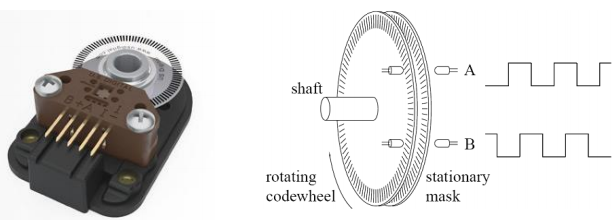
\includegraphics{images/fig3-3-encoder.PNG}
\end{figure}
Fig. 1: Example of a wheel encoder used to sum pulses and compute the
robot pose.

Such information is yielded by the firmware of the robotic base, which
computes it at very high rate (\emph{e.g.} at 100Hz) considering
constant linear \(v_t\) and angular \(w_t\) velocities, and makes it
available to the robot at lower rate (\emph{e.g.} 10Hz) using a tool
that we already know: the composition of poses.

\begin{figure}
\centering
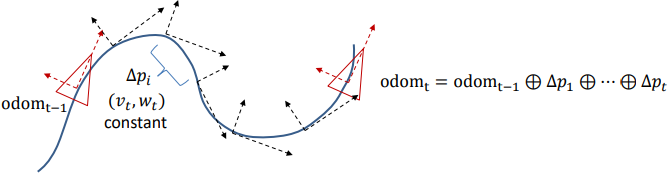
\includegraphics{images/fig3-3-odometry_compositions.PNG}
\end{figure}
Fig. 2: Example of composition of poses based on odometry.

The \textbf{odometry motion model} consists of the utilization of such
information that, although technically being a measurement rather than a
control, will be treated as a control command to simplify the modeling.
Thus, the odometry commands take the form of:

\[
    u_t = f(odom_t,odom_{t-1}) = \begin{bmatrix}
            \Delta x  \\
            \Delta y \\
            \Delta \theta
        \end{bmatrix}
\]

being \(odom_t\) and \(odom_{t-1}\) measurements taken as control and
computed from the odometry at time instants \(t\) and \(t-1\).

We will implement this motion model in two different forms: - Analytical
form: \(u_t=[\Delta x_t, \Delta y_t, \Delta \theta_t]^T\) - Sample form:
\(u_t=[\theta_1,d,\theta_2]^T\)

In this way, the utilization of the odometry motion model is more
suitable to keep track and estimate the robot pose in contrast to the
\emph{velocity model}.

    \begin{tcolorbox}[breakable, size=fbox, boxrule=1pt, pad at break*=1mm,colback=cellbackground, colframe=cellborder]
\prompt{In}{incolor}{1}{\boxspacing}
\begin{Verbatim}[commandchars=\\\{\}]
\PY{o}{\PYZpc{}}\PY{k}{matplotlib} notebook

\PY{c+c1}{\PYZsh{} IMPORTS}
\PY{k+kn}{import} \PY{n+nn}{numpy} \PY{k}{as} \PY{n+nn}{np}
\PY{k+kn}{from} \PY{n+nn}{numpy} \PY{k+kn}{import} \PY{n}{random}
\PY{k+kn}{import} \PY{n+nn}{matplotlib}\PY{n+nn}{.}\PY{n+nn}{pyplot} \PY{k}{as} \PY{n+nn}{plt}
\PY{k+kn}{from} \PY{n+nn}{scipy} \PY{k+kn}{import} \PY{n}{stats}

\PY{k+kn}{import} \PY{n+nn}{sys}
\PY{n}{sys}\PY{o}{.}\PY{n}{path}\PY{o}{.}\PY{n}{append}\PY{p}{(}\PY{l+s+s2}{\PYZdq{}}\PY{l+s+s2}{..}\PY{l+s+s2}{\PYZdq{}}\PY{p}{)}
\PY{k+kn}{from} \PY{n+nn}{utils}\PY{n+nn}{.}\PY{n+nn}{DrawRobot} \PY{k+kn}{import} \PY{n}{DrawRobot}
\PY{k+kn}{from} \PY{n+nn}{utils}\PY{n+nn}{.}\PY{n+nn}{PlotEllipse} \PY{k+kn}{import} \PY{n}{PlotEllipse}
\PY{k+kn}{from} \PY{n+nn}{utils}\PY{n+nn}{.}\PY{n+nn}{pause} \PY{k+kn}{import} \PY{n}{pause}
\PY{k+kn}{from} \PY{n+nn}{utils}\PY{n+nn}{.}\PY{n+nn}{Jacobians} \PY{k+kn}{import} \PY{n}{J1}\PY{p}{,} \PY{n}{J2}
\PY{k+kn}{from} \PY{n+nn}{utils}\PY{n+nn}{.}\PY{n+nn}{tcomp} \PY{k+kn}{import} \PY{n}{tcomp}
\end{Verbatim}
\end{tcolorbox}

    \hypertarget{analytic-form}{%
\subsection{3.3.1 Analytic form}\label{analytic-form}}

Just as we did in chapter 3.1, the analytic form of the odometry motion
model uses the composition of poses to model the robot's movement,
providing only a notion of how much the pose has changed, not how did it
get there.

As with the \emph{velocity model}, the odometry one uses a gaussian
distribution to represent the \textbf{robot pose}, so
\(x_t \sim(\overline{x}_t, \Sigma_{x_t})\), being its mean and
covariance computed as:

\begin{itemize}
\item
  \textbf{Mean:} \[\overline{x}_t 
  = 
  g(\overline{x}_{t-1},\overline{u}_t)
  = 
  \overline{x}_{t-1}\oplus \overline{u}_t \\[10pt]\] where
  \(u_t=[\Delta x_t, \Delta y_t, \Delta \theta_t]^T\), so: \(\\[10pt]\)
  \[
    g(\overline{x}_{t-1},\overline{u}_t)
    = \begin{bmatrix}
        x_1 + \Delta x \cos \theta_1 - \Delta y \sin \theta_1 \\ 
        y_1 + \Delta x \sin \theta_1 - \Delta y \cos \theta_1 \\
        \theta_1 + \Delta \theta
      \end{bmatrix}
  \]
\item
  \textbf{Covariance:} \$\$\Sigma\emph{\{x\_t\} =\\
  \frac{\partial g}{\partial x_{t-1}} \cdot \Sigma}\{x\_\{t-1\}\}
  \cdot {\frac{\partial g}{\partial x_{t-1}}}\^{}T
\item
  \frac{\partial g}{\partial u_{t}} \cdot \Sigma\_\{u\_t\}
  \cdot {\frac{\partial g}{\partial u_{t}}}\^{}T
  \textbackslash{[}10pt{]}\[
  where $\partial g / \partial x_{t-1}$ and $\partial g / \partial u_{t}$ are the jacobians of our motion model evaluated at the previous pose $x_{t-1}$ and the current command $u_t$:
  \] \frac{\partial g}{\partial x_{k-1}} =

  \begin{bmatrix}
    1 & 0 & -\Delta x_k \sin \theta_{k-1}-\Delta y_k \cos \theta_{k-1} \\
    0 & 1 & \Delta x_k \cos \theta_{k-1} - \Delta y_k \sin \theta_{k-1} \\
    0 & 0 & 1
    \end{bmatrix}

  , , , , , , , , , , , , \frac{\partial g}{\partial u_k} =

  \begin{bmatrix}
    \cos \theta_{k-1} & -\sin \theta_{k-1} & 0  \\
    \sin \theta_{k-1} & \cos \theta_{k-1} & 0 \\
    0 & 0 & 1
    \end{bmatrix}

  \textbackslash{[}10pt{]} \[
  and the covariance matrix of this movement ($\Sigma_{u_t}$) is defined as seen below. Typically, it is constant during robot motion:$\\[10pt]$
  \] \Sigma\_\{u\_t\} =

  \begin{bmatrix}
            \sigma_{\Delta x}^2 & 0 & 0\\
            0 &  \sigma_{\Delta y}^2 & 0 \\
            0 & 0 &  \sigma_{\Delta \theta}^2 
        \end{bmatrix}

  \$\$
\end{itemize}

    \hypertarget{assignment-1-the-model-in-action}{%
\subsubsection{\texorpdfstring{\textbf{{ASSIGNMENT 1: The model in
action}}}{ASSIGNMENT 1: The model in action}}\label{assignment-1-the-model-in-action}}

Similarly to the assignment 3.1, we'll move a robot along a 8-by-8
square (in meters), in increments of 2m. In this case you have to
complete:

\begin{itemize}
\tightlist
\item
  The \texttt{step()} method to compute:

  \begin{itemize}
  \tightlist
  \item
    the new expected pose (\texttt{self.pose}),
  \item
    the new true pose \(x_t\) (ground-truth \texttt{self.true\_pose})
    after adding some noise using
    \href{https://docs.scipy.org/doc/scipy/reference/generated/scipy.stats.multivariate_normal.html}{\texttt{stats.multivariate\_normal.rvs()}}
    to the movement command \(u\) according to \texttt{Q} (which
    represents \(\Sigma_{u_t}\)),
  \item
    and to update the uncertainty about the robot position in
    \texttt{self.P} (covariance matrix \(\Sigma_{x_t}\)). Note that the
    methods \texttt{J1()} and \texttt{J2()} already implement
    \(\partial g / \partial x_{t-1}\) and
    \(\partial g / \partial u_{t}\) for you, you just have to call them
    with the right input parameters.
  \end{itemize}
\item
  The \texttt{draw()} method to plot:

  \begin{itemize}
  \tightlist
  \item
    the uncertainty of the pose as an ellipse centered at the expected
    pose, and
  \item
    the true position (ground-truth).
  \end{itemize}
\end{itemize}

We are going to consider the following motion covariance matrix (it is
already coded for you):

\[
    \Sigma_{u_t} = \begin{bmatrix}
        0.04 & 0 & 0 \\
        0 & 0.04 & 0 \\
        0 & 0 & 0.01
    \end{bmatrix}
\]

\textbf{Example}


\begin{figure}
\centering
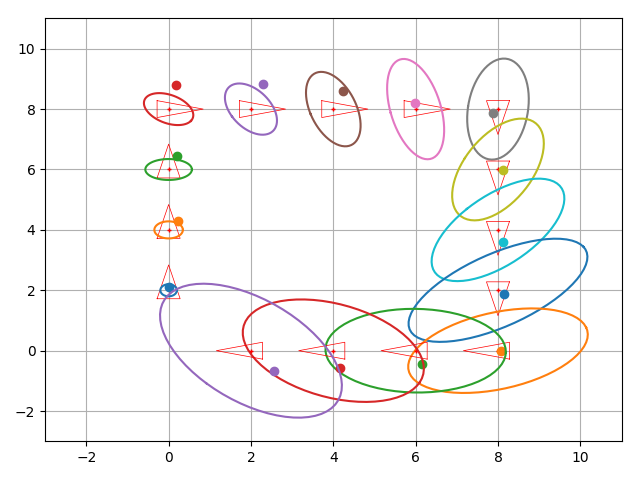
\includegraphics{images/fig3-3-1.PNG}
\end{figure}
Fig. 2: Movement of a robot using odometry commands. Representing the
expected pose (in red), the true pose (as dots) and the confidence
ellipse.

    \begin{tcolorbox}[breakable, size=fbox, boxrule=1pt, pad at break*=1mm,colback=cellbackground, colframe=cellborder]
\prompt{In}{incolor}{18}{\boxspacing}
\begin{Verbatim}[commandchars=\\\{\}]
\PY{k}{class} \PY{n+nc}{Robot}\PY{p}{(}\PY{p}{)}\PY{p}{:}
    \PY{l+s+sd}{\PYZdq{}\PYZdq{}\PYZdq{} Simulation of a robot base}
\PY{l+s+sd}{    }
\PY{l+s+sd}{        Attrs:}
\PY{l+s+sd}{            pose: Expected pose of the robot}
\PY{l+s+sd}{            P: Covariance of the current pose}
\PY{l+s+sd}{            true\PYZus{}pose: Real pose of the robot(affected by noise)}
\PY{l+s+sd}{            Q: Covariance of the movement}
\PY{l+s+sd}{    \PYZdq{}\PYZdq{}\PYZdq{}}
    \PY{k}{def} \PY{n+nf+fm}{\PYZus{}\PYZus{}init\PYZus{}\PYZus{}}\PY{p}{(}\PY{n+nb+bp}{self}\PY{p}{,} \PY{n}{x}\PY{p}{,} \PY{n}{P}\PY{p}{,} \PY{n}{Q}\PY{p}{)}\PY{p}{:}
        \PY{n+nb+bp}{self}\PY{o}{.}\PY{n}{pose} \PY{o}{=} \PY{n}{x}
        \PY{n+nb+bp}{self}\PY{o}{.}\PY{n}{P} \PY{o}{=} \PY{n}{P}
        \PY{n+nb+bp}{self}\PY{o}{.}\PY{n}{true\PYZus{}pose} \PY{o}{=} \PY{n+nb+bp}{self}\PY{o}{.}\PY{n}{pose}
        \PY{n+nb+bp}{self}\PY{o}{.}\PY{n}{Q} \PY{o}{=} \PY{n}{Q}
        
    \PY{k}{def} \PY{n+nf}{step}\PY{p}{(}\PY{n+nb+bp}{self}\PY{p}{,} \PY{n}{u}\PY{p}{)}\PY{p}{:}
        \PY{c+c1}{\PYZsh{} TODO Update expected pose}
        \PY{n}{prev\PYZus{}pose} \PY{o}{=} \PY{n+nb+bp}{self}\PY{o}{.}\PY{n}{pose}
        \PY{n+nb+bp}{self}\PY{o}{.}\PY{n}{pose} \PY{o}{=} \PY{n}{tcomp}\PY{p}{(}\PY{n}{prev\PYZus{}pose}\PY{p}{,} \PY{n}{u}\PY{p}{)}
        
        \PY{c+c1}{\PYZsh{} TODO Generate true pose }
        \PY{n}{noisy\PYZus{}u} \PY{o}{=} \PY{n}{np}\PY{o}{.}\PY{n}{vstack}\PY{p}{(}\PY{n}{stats}\PY{o}{.}\PY{n}{multivariate\PYZus{}normal}\PY{o}{.}\PY{n}{rvs}\PY{p}{(}\PY{n}{mean}\PY{o}{=}\PY{n}{u}\PY{o}{.}\PY{n}{flatten}\PY{p}{(}\PY{p}{)}\PY{p}{,} \PY{n}{cov}\PY{o}{=}\PY{n+nb+bp}{self}\PY{o}{.}\PY{n}{Q}\PY{p}{)}\PY{p}{)}
        \PY{n+nb+bp}{self}\PY{o}{.}\PY{n}{true\PYZus{}pose} \PY{o}{=} \PY{n}{tcomp}\PY{p}{(}\PY{n+nb+bp}{self}\PY{o}{.}\PY{n}{true\PYZus{}pose}\PY{p}{,} \PY{n}{noisy\PYZus{}u}\PY{p}{)}
        
        \PY{c+c1}{\PYZsh{}\PYZsh{} Preguntar \PYZsh{}\PYZsh{}}
        \PY{c+c1}{\PYZsh{} TODO Update covariance}
        \PY{n}{JacF\PYZus{}x} \PY{o}{=} \PY{n}{J1}\PY{p}{(}\PY{n}{prev\PYZus{}pose}\PY{p}{,} \PY{n}{u}\PY{p}{)}
        \PY{n}{JacF\PYZus{}u} \PY{o}{=} \PY{n}{J2}\PY{p}{(}\PY{n}{prev\PYZus{}pose}\PY{p}{,} \PY{n}{u}\PY{p}{)}

        \PY{n+nb+bp}{self}\PY{o}{.}\PY{n}{P} \PY{o}{=} \PY{p}{(}
            \PY{p}{(}\PY{n}{JacF\PYZus{}x} \PY{o}{@} \PY{n+nb+bp}{self}\PY{o}{.}\PY{n}{P} \PY{o}{@} \PY{n}{JacF\PYZus{}x}\PY{o}{.}\PY{n}{T}\PY{p}{)} 
            \PY{o}{+} \PY{p}{(}\PY{n}{JacF\PYZus{}u} \PY{o}{@} \PY{n+nb+bp}{self}\PY{o}{.}\PY{n}{Q} \PY{o}{@} \PY{n}{JacF\PYZus{}u}\PY{o}{.}\PY{n}{T}\PY{p}{)}
        \PY{p}{)}
        
    
    \PY{k}{def} \PY{n+nf}{draw}\PY{p}{(}\PY{n+nb+bp}{self}\PY{p}{,} \PY{n}{fig}\PY{p}{,} \PY{n}{ax}\PY{p}{)}\PY{p}{:}
        \PY{n}{DrawRobot}\PY{p}{(}\PY{n}{fig}\PY{p}{,} \PY{n}{ax}\PY{p}{,} \PY{n+nb+bp}{self}\PY{o}{.}\PY{n}{pose}\PY{p}{)}
        \PY{n}{el} \PY{o}{=} \PY{n}{PlotEllipse}\PY{p}{(}\PY{n}{fig}\PY{p}{,} \PY{n}{ax}\PY{p}{,} \PY{n+nb+bp}{self}\PY{o}{.}\PY{n}{pose}\PY{p}{,} \PY{n+nb+bp}{self}\PY{o}{.}\PY{n}{P}\PY{p}{)}
        \PY{n}{ax}\PY{o}{.}\PY{n}{plot}\PY{p}{(}\PY{n+nb+bp}{self}\PY{o}{.}\PY{n}{true\PYZus{}pose}\PY{p}{[}\PY{l+m+mi}{0}\PY{p}{,}\PY{l+m+mi}{0}\PY{p}{]}\PY{p}{,} \PY{n+nb+bp}{self}\PY{o}{.}\PY{n}{true\PYZus{}pose}\PY{p}{[}\PY{l+m+mi}{1}\PY{p}{,}\PY{l+m+mi}{0}\PY{p}{]}\PY{p}{,} \PY{l+s+s1}{\PYZsq{}}\PY{l+s+s1}{o}\PY{l+s+s1}{\PYZsq{}}\PY{p}{,} \PY{n}{color}\PY{o}{=}\PY{n}{el}\PY{p}{[}\PY{l+m+mi}{0}\PY{p}{]}\PY{o}{.}\PY{n}{get\PYZus{}color}\PY{p}{(}\PY{p}{)}\PY{p}{)}
  
\end{Verbatim}
\end{tcolorbox}

    You can use the following demo to \textbf{try your new \texttt{Robot()}
class}.

    \begin{tcolorbox}[breakable, size=fbox, boxrule=1pt, pad at break*=1mm,colback=cellbackground, colframe=cellborder]
\prompt{In}{incolor}{3}{\boxspacing}
\begin{Verbatim}[commandchars=\\\{\}]
\PY{k}{def} \PY{n+nf}{demo\PYZus{}odometry\PYZus{}commands\PYZus{}analytical}\PY{p}{(}\PY{n}{robot}\PY{p}{)}\PY{p}{:}  
    \PY{c+c1}{\PYZsh{} MATPLOTLIB}
    \PY{n}{fig}\PY{p}{,} \PY{n}{ax} \PY{o}{=} \PY{n}{plt}\PY{o}{.}\PY{n}{subplots}\PY{p}{(}\PY{p}{)}
    \PY{n}{ax}\PY{o}{.}\PY{n}{set\PYZus{}xlim}\PY{p}{(}\PY{p}{[}\PY{o}{\PYZhy{}}\PY{l+m+mi}{3}\PY{p}{,} \PY{l+m+mi}{11}\PY{p}{]}\PY{p}{)}
    \PY{n}{ax}\PY{o}{.}\PY{n}{set\PYZus{}ylim}\PY{p}{(}\PY{p}{[}\PY{o}{\PYZhy{}}\PY{l+m+mi}{3}\PY{p}{,} \PY{l+m+mi}{11}\PY{p}{]}\PY{p}{)}
    \PY{n}{plt}\PY{o}{.}\PY{n}{ion}\PY{p}{(}\PY{p}{)}
    \PY{n}{plt}\PY{o}{.}\PY{n}{grid}\PY{p}{(}\PY{p}{)}
    \PY{n}{plt}\PY{o}{.}\PY{n}{tight\PYZus{}layout}\PY{p}{(}\PY{p}{)}
    \PY{n}{fig}\PY{o}{.}\PY{n}{canvas}\PY{o}{.}\PY{n}{draw}\PY{p}{(}\PY{p}{)}
    
    \PY{c+c1}{\PYZsh{} MOVEMENT PARAMETERS}
    \PY{n}{nSteps} \PY{o}{=} \PY{l+m+mi}{15}
    \PY{n}{ang} \PY{o}{=} \PY{o}{\PYZhy{}}\PY{n}{np}\PY{o}{.}\PY{n}{pi}\PY{o}{/}\PY{l+m+mi}{2} \PY{c+c1}{\PYZsh{} angle to turn in corners}
    \PY{n}{u} \PY{o}{=} \PY{n}{np}\PY{o}{.}\PY{n}{vstack}\PY{p}{(}\PY{p}{(}\PY{l+m+mf}{2.}\PY{p}{,} \PY{l+m+mf}{0.}\PY{p}{,} \PY{l+m+mf}{0.}\PY{p}{)}\PY{p}{)}
    
    \PY{c+c1}{\PYZsh{} MAIN LOOP}
    \PY{k}{for} \PY{n}{i} \PY{o+ow}{in} \PY{n+nb}{range}\PY{p}{(}\PY{n}{nSteps}\PY{p}{)}\PY{p}{:}
        \PY{c+c1}{\PYZsh{} change angle on corners}
        \PY{k}{if} \PY{n}{i} \PY{o}{\PYZpc{}} \PY{l+m+mi}{4} \PY{o}{==} \PY{l+m+mi}{3}\PY{p}{:}
            \PY{n}{u}\PY{p}{[}\PY{l+m+mi}{2}\PY{p}{,} \PY{l+m+mi}{0}\PY{p}{]} \PY{o}{=} \PY{n}{ang}

        \PY{c+c1}{\PYZsh{}Update positions}
        \PY{n}{robot}\PY{o}{.}\PY{n}{step}\PY{p}{(}\PY{n}{u}\PY{p}{)}

        \PY{c+c1}{\PYZsh{} Restore angle iff changed}
        \PY{k}{if} \PY{n}{i} \PY{o}{\PYZpc{}} \PY{l+m+mi}{4} \PY{o}{==} \PY{l+m+mi}{3}\PY{p}{:}
            \PY{n}{u}\PY{p}{[}\PY{l+m+mi}{2}\PY{p}{,} \PY{l+m+mi}{0}\PY{p}{]} \PY{o}{=} \PY{l+m+mi}{0}

        \PY{c+c1}{\PYZsh{} Draw every loop}
        \PY{n}{robot}\PY{o}{.}\PY{n}{draw}\PY{p}{(}\PY{n}{fig}\PY{p}{,} \PY{n}{ax}\PY{p}{)}
        \PY{n}{fig}\PY{o}{.}\PY{n}{canvas}\PY{o}{.}\PY{n}{draw}\PY{p}{(}\PY{p}{)}
        \PY{n}{plt}\PY{o}{.}\PY{n}{pause}\PY{p}{(}\PY{l+m+mf}{0.3}\PY{p}{)}
\end{Verbatim}
\end{tcolorbox}

    \begin{tcolorbox}[breakable, size=fbox, boxrule=1pt, pad at break*=1mm,colback=cellbackground, colframe=cellborder]
\prompt{In}{incolor}{19}{\boxspacing}
\begin{Verbatim}[commandchars=\\\{\}]
\PY{c+c1}{\PYZsh{}\PYZsh{} PREGUNTAR \PYZsh{}\PYZsh{}}
\PY{n}{x} \PY{o}{=} \PY{n}{np}\PY{o}{.}\PY{n}{vstack}\PY{p}{(}\PY{p}{[}\PY{l+m+mf}{0.}\PY{p}{,} \PY{l+m+mf}{0.}\PY{p}{,} \PY{n}{np}\PY{o}{.}\PY{n}{pi}\PY{o}{/}\PY{l+m+mi}{2}\PY{p}{]}\PY{p}{)} \PY{c+c1}{\PYZsh{} pose inicial}

\PY{c+c1}{\PYZsh{} Probabilistic parameters}
\PY{n}{P} \PY{o}{=} \PY{n}{np}\PY{o}{.}\PY{n}{diag}\PY{p}{(}\PY{p}{[}\PY{l+m+mf}{0.}\PY{p}{,} \PY{l+m+mf}{0.}\PY{p}{,} \PY{l+m+mf}{0.}\PY{p}{]}\PY{p}{)}
\PY{n}{Q} \PY{o}{=} \PY{n}{np}\PY{o}{.}\PY{n}{diag}\PY{p}{(}\PY{p}{[}\PY{l+m+mf}{0.04}\PY{p}{,} \PY{l+m+mf}{0.04}\PY{p}{,} \PY{l+m+mf}{0.01}\PY{p}{]}\PY{p}{)}

\PY{n}{robot} \PY{o}{=} \PY{n}{Robot}\PY{p}{(}\PY{n}{x}\PY{p}{,} \PY{n}{P}\PY{p}{,} \PY{n}{Q}\PY{p}{)}
\PY{n}{demo\PYZus{}odometry\PYZus{}commands\PYZus{}analytical}\PY{p}{(}\PY{n}{robot}\PY{p}{)}
\end{Verbatim}
\end{tcolorbox}

\begin{figure}
\centering
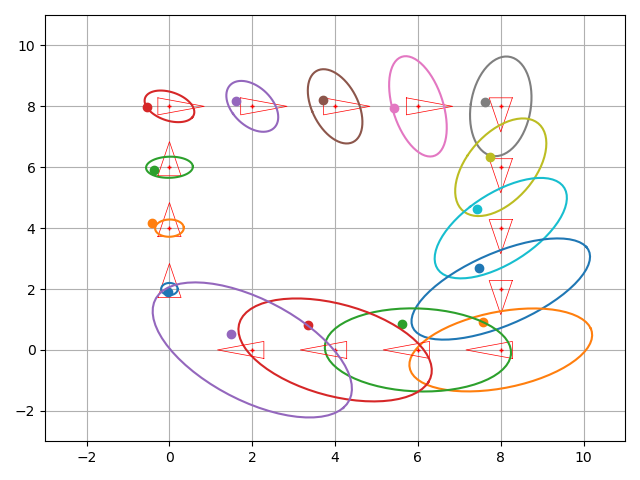
\includegraphics{returns/331_2.PNG}
\end{figure}
    
    \hypertarget{thinking-about-it-1}{%
\subsubsection{Thinking about it (1)}\label{thinking-about-it-1}}

Once you have completed this assignment regarding the analytical form of
the odometry model, \textbf{answer the following questions}:

\begin{itemize}
\item
  Which is the difference between the \(g(\cdot)\) function used here,
  and the one in the velocity model?

  In the Velocity Based motion model, we use the old pose and the
  velocity of the robot meanwhile in the Odometry Based motion model, we
  use the old pose and the movement we want to do.
\item
  How many parameters compound the motion command \(u_t\) in this model?

  Three. X and Y coords and the angle.
\item
  Which is the role of the Jacobians \(\partial g / \partial x_{t-1}\)
  and \(\partial g / \partial u_{t}\)?

  Jacobians are used to obtain the new value of the covariance. (Noise
  propagated)
\item
  What happens if you modify the covariance matrix \(\Sigma_{u_t}\)
  modeling the uncertainty in the motion command \(u_t\)? Try different
  values and discuss the results.

  If we increase the values of the covariance matrix, the real\_pose
  will probably be more dispersed from the mean. If we decrease them,
  the real\_pose will probably be near the mean.
\end{itemize}

    \hypertarget{sample-form}{%
\subsection{3.3.2 Sample form}\label{sample-form}}

The analytical form used above, although useful for the probabilistic
algorithms we will cover in this course, does not work well for sampling
algorithms such as particle filters.

The reason being, if we generate random samples from the gaussian
distributions as in the previous exercise, we will find some poses that
are not feasible to the non-holonomic movement of a robot, i.e.~they do
not correspond to a velocity command \((v, w)\) with noise.

The following \emph{sample form} is a more realistic way to generate
samples of the robot pose. In this case, the movement of the robot is
modeled as a sequence of actions (see Fig 3):

\begin{enumerate}
\def\labelenumi{\arabic{enumi}.}
\tightlist
\item
  \textbf{Turn} (\(\theta_1\)): to face the destination point.
\item
  \textbf{Advance} (\(d\)): to arrive at the destination.
\item
  \textbf{Turn} (\(\theta_2\)): to get to the desired angle.
\end{enumerate}


\begin{figure}
\centering
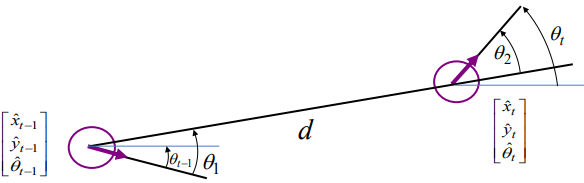
\includegraphics{images/fig3-3-odometry_sample_form.PNG}
\end{figure}
Fig. 3: Movement of a robot using odometry commands in sampling form.

So this type of order is expressed as:

\[
    u_t = \begin{bmatrix}
            \theta_1  \\
            d \\
            \theta_2
        \end{bmatrix}
\]

It can easily be generated from odometry poses
\([\hat x_t, \hat y_t,\hat \theta_t]^T\) and
\([\hat x_{t-1}, \hat y_{t-1},\hat \theta_{t-1}]^T\) given the following
equations:

\[
    \begin{equation}
    \theta_1 =atan2(\hat y_t -\hat y_{t-1}, \hat x_t -\hat x_{t-1})- \hat \theta_{t-1} \\
    d = \sqrt{(\hat y_t -\hat y_{t-1})^2 + (\hat x_t -\hat x_{t-1})^2} \\
    \theta_2  = \hat{\theta}_t - \hat{\theta}_{t-1} - \theta_1
    \end{equation}
\]

    \hypertarget{assignment-2-implementing-the-sampling-form}{%
\subsubsection{\texorpdfstring{\textbf{{ASSIGNMENT 2: Implementing the
sampling
form}}}{ASSIGNMENT 2: Implementing the sampling form}}\label{assignment-2-implementing-the-sampling-form}}

Complete the following cells to experience the motion of a robot using
the sampling form of the odometry model. For that:

\begin{enumerate}
\def\labelenumi{\arabic{enumi}.}
\tightlist
\item
  Implement a function that, given the previously mentioned
  \([\hat x_t, \hat y_t,\hat \theta_t]^T\) and
  \([\hat x_{t-1}, \hat y_{t-1},\hat \theta_{t-1}]^T\) generates an
  order \(u_t = [ \theta_1, d , \theta_2 ]^T\)
\end{enumerate}

    \begin{tcolorbox}[breakable, size=fbox, boxrule=1pt, pad at break*=1mm,colback=cellbackground, colframe=cellborder]
\prompt{In}{incolor}{5}{\boxspacing}
\begin{Verbatim}[commandchars=\\\{\}]
\PY{k}{def} \PY{n+nf}{generate\PYZus{}move}\PY{p}{(}\PY{n}{pose\PYZus{}now}\PY{p}{,} \PY{n}{pose\PYZus{}old}\PY{p}{)}\PY{p}{:}
    \PY{n}{diff} \PY{o}{=} \PY{n}{pose\PYZus{}now} \PY{o}{\PYZhy{}} \PY{n}{pose\PYZus{}old}
    \PY{n}{theta1} \PY{o}{=} \PY{n}{np}\PY{o}{.}\PY{n}{arctan2}\PY{p}{(}\PY{n}{pose\PYZus{}now}\PY{p}{[}\PY{l+m+mi}{1}\PY{p}{]}\PY{o}{\PYZhy{}}\PY{n}{pose\PYZus{}old}\PY{p}{[}\PY{l+m+mi}{1}\PY{p}{]}\PY{p}{,} \PY{n}{pose\PYZus{}now}\PY{p}{[}\PY{l+m+mi}{0}\PY{p}{]}\PY{o}{\PYZhy{}}\PY{n}{pose\PYZus{}old}\PY{p}{[}\PY{l+m+mi}{0}\PY{p}{]}\PY{p}{)} \PY{o}{\PYZhy{}} \PY{n}{pose\PYZus{}old}\PY{p}{[}\PY{l+m+mi}{2}\PY{p}{]}
    \PY{n}{d} \PY{o}{=} \PY{n}{np}\PY{o}{.}\PY{n}{sqrt}\PY{p}{(}\PY{p}{(}\PY{n}{pose\PYZus{}now}\PY{p}{[}\PY{l+m+mi}{1}\PY{p}{]}\PY{o}{\PYZhy{}}\PY{n}{pose\PYZus{}old}\PY{p}{[}\PY{l+m+mi}{1}\PY{p}{]}\PY{p}{)}\PY{o}{*}\PY{o}{*}\PY{l+m+mi}{2} \PY{o}{+} \PY{p}{(}\PY{n}{pose\PYZus{}now}\PY{p}{[}\PY{l+m+mi}{0}\PY{p}{]}\PY{o}{\PYZhy{}}\PY{n}{pose\PYZus{}old}\PY{p}{[}\PY{l+m+mi}{0}\PY{p}{]}\PY{p}{)}\PY{o}{*}\PY{o}{*}\PY{l+m+mi}{2}\PY{p}{)}
    \PY{n}{theta2} \PY{o}{=} \PY{n}{pose\PYZus{}now}\PY{p}{[}\PY{l+m+mi}{2}\PY{p}{]} \PY{o}{\PYZhy{}} \PY{n}{pose\PYZus{}old}\PY{p}{[}\PY{l+m+mi}{2}\PY{p}{]} \PY{o}{\PYZhy{}} \PY{n}{theta1}
    \PY{k}{return} \PY{n}{np}\PY{o}{.}\PY{n}{vstack}\PY{p}{(}\PY{p}{(}\PY{n}{theta1}\PY{p}{,} \PY{n}{d}\PY{p}{,} \PY{n}{theta2}\PY{p}{)}\PY{p}{)}
\end{Verbatim}
\end{tcolorbox}

    \textbf{Try such function} with the code cell below:

    \begin{tcolorbox}[breakable, size=fbox, boxrule=1pt, pad at break*=1mm,colback=cellbackground, colframe=cellborder]
\prompt{In}{incolor}{6}{\boxspacing}
\begin{Verbatim}[commandchars=\\\{\}]
\PY{n}{generate\PYZus{}move}\PY{p}{(}\PY{n}{np}\PY{o}{.}\PY{n}{vstack}\PY{p}{(}\PY{p}{[}\PY{l+m+mf}{0.}\PY{p}{,} \PY{l+m+mf}{0.}\PY{p}{,} \PY{l+m+mf}{0.}\PY{p}{]}\PY{p}{)}\PY{p}{,} \PY{n}{np}\PY{o}{.}\PY{n}{vstack}\PY{p}{(}\PY{p}{[}\PY{l+m+mf}{1.}\PY{p}{,} \PY{l+m+mf}{1.}\PY{p}{,} \PY{n}{np}\PY{o}{.}\PY{n}{pi}\PY{o}{/}\PY{l+m+mi}{2}\PY{p}{]}\PY{p}{)}\PY{p}{)}
\end{Verbatim}
\end{tcolorbox}

            \begin{tcolorbox}[breakable, size=fbox, boxrule=.5pt, pad at break*=1mm, opacityfill=0]
\prompt{Out}{outcolor}{6}{\boxspacing}
\begin{Verbatim}[commandchars=\\\{\}]
array([[-3.92699082],
       [ 1.41421356],
       [ 2.35619449]])
\end{Verbatim}
\end{tcolorbox}
        
    Expected output for the commented example:

\begin{verbatim}
array([[-3.92699082],
     [ 1.41421356],
     [ 2.35619449]])
\end{verbatim}

    \begin{enumerate}
\def\labelenumi{\arabic{enumi}.}
\setcounter{enumi}{1}
\tightlist
\item
  Using the resulting control action
  \(u_t = [\hat \theta_1, \hat d, \hat \theta_2]^T\) we can model its
  noise in the following way:
\end{enumerate}

\[
    \begin{equation}
        \theta_1 = \hat\theta_1 + \text{sample}\left(\alpha_0 \hat\theta_1^2 + \alpha_1 \hat d^2 \right) \\
        d = \hat d + \text{sample}\left(\alpha_2 \hat d^2 + \alpha_3 \left(\hat\theta_1^2 + \hat d^2 \right) \right) \\
        \theta_2 = \hat\theta_2 + \text{sample}\left(\alpha_0 \hat\theta_2^2 + \alpha_1 \hat d^2\right)
    \end{equation}
  \]

Where \(sample(b)\) generates a random value from a distribution
\(N(0, b)\). The vector \(\alpha = [\alpha_0, \dots, \alpha_3]\)
(\texttt{a} in the code), models the robot's intrinsic noise.

The pose of the robot at the end of the movement is computed as follows:
\[
    \begin{equation}
        x_t = x_{t-1} + d \cos\left(\theta_{t-1} + \theta_1 \right) \\
        y_t = y_{t-1} + d \sin\left(\theta_{t-1} + \theta_1 \right) \\
        \theta_t = \theta_{t-1} +  \theta_1 +  \theta_2
    \end{equation}
\] Complete the \texttt{step()} and \texttt{draw()} methods to: - Update
the expected robot pose (\texttt{self.pose}) and generate new samples.
The number of samples is set by \texttt{n\_samples}, and
\texttt{self.samples} is in charge of storing such samples. Each sample
can be interpreted as one possible pose reached by the robot. - Draw the
true pose of the robot (without angle) as a cloud of particles (samples
of possible points which the robot can be at). Play a bit with different
values of \texttt{a}. To improve this visualization the robot will move
in increments of \(0.5\) and we are going to plot the particles each 4
increments.

\textbf{Example}

\begin{figure}
\centering
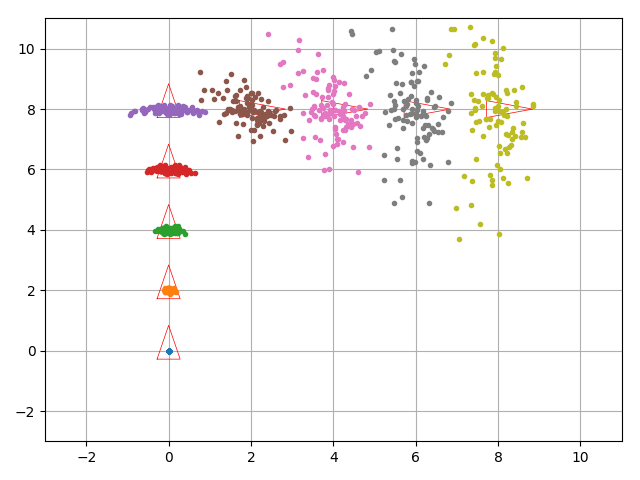
\includegraphics{images/fig3-3-2.PNG}
\end{figure}
Fig. 1: Movement of a robot using odometry commands in sampling form.
Representing the expected pose (in red) and the samples (as clouds of
dots)

    \begin{tcolorbox}[breakable, size=fbox, boxrule=1pt, pad at break*=1mm,colback=cellbackground, colframe=cellborder]
\prompt{In}{incolor}{7}{\boxspacing}
\begin{Verbatim}[commandchars=\\\{\}]
\PY{k}{class} \PY{n+nc}{SampledRobot}\PY{p}{(}\PY{n+nb}{object}\PY{p}{)}\PY{p}{:}
    \PY{k}{def} \PY{n+nf+fm}{\PYZus{}\PYZus{}init\PYZus{}\PYZus{}}\PY{p}{(}\PY{n+nb+bp}{self}\PY{p}{,} \PY{n}{mean}\PY{p}{,} \PY{n}{a}\PY{p}{,} \PY{n}{n\PYZus{}samples}\PY{p}{)}\PY{p}{:}
        \PY{n+nb+bp}{self}\PY{o}{.}\PY{n}{pose} \PY{o}{=} \PY{n}{mean}
        \PY{n+nb+bp}{self}\PY{o}{.}\PY{n}{a} \PY{o}{=} \PY{n}{a}
        \PY{n+nb+bp}{self}\PY{o}{.}\PY{n}{samples} \PY{o}{=} \PY{n}{np}\PY{o}{.}\PY{n}{tile}\PY{p}{(}\PY{n}{mean}\PY{p}{,} \PY{n}{n\PYZus{}samples}\PY{p}{)}
        
    \PY{k}{def} \PY{n+nf}{step}\PY{p}{(}\PY{n+nb+bp}{self}\PY{p}{,} \PY{n}{u}\PY{p}{)}\PY{p}{:}
        \PY{c+c1}{\PYZsh{} TODO Update pose}
        \PY{n}{ang} \PY{o}{=} \PY{n+nb+bp}{self}\PY{o}{.}\PY{n}{pose}\PY{p}{[}\PY{l+m+mi}{2}\PY{p}{,} \PY{l+m+mi}{0}\PY{p}{]} \PY{o}{+} \PY{n}{u}\PY{p}{[}\PY{l+m+mi}{0}\PY{p}{,} \PY{l+m+mi}{0}\PY{p}{]}
        \PY{n+nb+bp}{self}\PY{o}{.}\PY{n}{pose}\PY{p}{[}\PY{l+m+mi}{0}\PY{p}{,} \PY{l+m+mi}{0}\PY{p}{]} \PY{o}{+}\PY{o}{=} \PY{n}{u}\PY{p}{[}\PY{l+m+mi}{1}\PY{p}{,} \PY{l+m+mi}{0}\PY{p}{]} \PY{o}{*} \PY{n}{np}\PY{o}{.}\PY{n}{cos}\PY{p}{(}\PY{n}{ang}\PY{p}{)}
        \PY{n+nb+bp}{self}\PY{o}{.}\PY{n}{pose}\PY{p}{[}\PY{l+m+mi}{1}\PY{p}{,} \PY{l+m+mi}{0}\PY{p}{]} \PY{o}{+}\PY{o}{=} \PY{n}{u}\PY{p}{[}\PY{l+m+mi}{1}\PY{p}{,} \PY{l+m+mi}{0}\PY{p}{]} \PY{o}{*} \PY{n}{np}\PY{o}{.}\PY{n}{sin}\PY{p}{(}\PY{n}{ang}\PY{p}{)}
        \PY{n+nb+bp}{self}\PY{o}{.}\PY{n}{pose}\PY{p}{[}\PY{l+m+mi}{2}\PY{p}{,} \PY{l+m+mi}{0}\PY{p}{]} \PY{o}{=} \PY{n}{u}\PY{p}{[}\PY{l+m+mi}{2}\PY{p}{,} \PY{l+m+mi}{0}\PY{p}{]} \PY{o}{+} \PY{n}{ang}
                
        \PY{c+c1}{\PYZsh{} TODO Generate new samples}
        \PY{n}{sample} \PY{o}{=} \PY{k}{lambda} \PY{n}{b}\PY{p}{:} \PY{n}{stats}\PY{o}{.}\PY{n}{norm}\PY{p}{(}\PY{n}{loc}\PY{o}{=}\PY{l+m+mi}{0}\PY{p}{,} \PY{n}{scale}\PY{o}{=}\PY{n}{b}\PY{p}{)}\PY{o}{.}\PY{n}{rvs}\PY{p}{(}\PY{n}{size}\PY{o}{=}\PY{n+nb+bp}{self}\PY{o}{.}\PY{n}{samples}\PY{o}{.}\PY{n}{shape}\PY{p}{[}\PY{l+m+mi}{1}\PY{p}{]}\PY{p}{)}
        
        \PY{n}{u2} \PY{o}{=} \PY{n}{u}\PY{o}{*}\PY{o}{*}\PY{l+m+mi}{2}
        
        \PY{n}{noisy\PYZus{}u} \PY{o}{=} \PY{n}{u} \PY{o}{+} \PY{n}{np}\PY{o}{.}\PY{n}{vstack}\PY{p}{(}\PY{p}{(}
            \PY{n}{sample}\PY{p}{(}\PY{n+nb+bp}{self}\PY{o}{.}\PY{n}{a}\PY{p}{[}\PY{l+m+mi}{0}\PY{p}{]} \PY{o}{*} \PY{n}{u2}\PY{p}{[}\PY{l+m+mi}{0}\PY{p}{,} \PY{l+m+mi}{0}\PY{p}{]} \PY{o}{+} \PY{n+nb+bp}{self}\PY{o}{.}\PY{n}{a}\PY{p}{[}\PY{l+m+mi}{1}\PY{p}{]} \PY{o}{*} \PY{n}{u2}\PY{p}{[}\PY{l+m+mi}{1}\PY{p}{,} \PY{l+m+mi}{0}\PY{p}{]}\PY{p}{)}\PY{p}{,}
            \PY{n}{sample}\PY{p}{(}\PY{n+nb+bp}{self}\PY{o}{.}\PY{n}{a}\PY{p}{[}\PY{l+m+mi}{2}\PY{p}{]}\PY{o}{*}\PY{n}{u2}\PY{p}{[}\PY{l+m+mi}{1}\PY{p}{,} \PY{l+m+mi}{0}\PY{p}{]} \PY{o}{+} \PY{n+nb+bp}{self}\PY{o}{.}\PY{n}{a}\PY{p}{[}\PY{l+m+mi}{3}\PY{p}{]} \PY{o}{*} \PY{p}{(}\PY{n}{u2}\PY{p}{[}\PY{l+m+mi}{0}\PY{p}{,} \PY{l+m+mi}{0}\PY{p}{]} \PY{o}{+} \PY{n}{u2}\PY{p}{[}\PY{l+m+mi}{1}\PY{p}{,} \PY{l+m+mi}{0}\PY{p}{]}\PY{p}{)}\PY{p}{)}\PY{p}{,}
            \PY{n}{sample}\PY{p}{(}\PY{n+nb+bp}{self}\PY{o}{.}\PY{n}{a}\PY{p}{[}\PY{l+m+mi}{0}\PY{p}{]} \PY{o}{*} \PY{n}{u2}\PY{p}{[}\PY{l+m+mi}{2}\PY{p}{,} \PY{l+m+mi}{0}\PY{p}{]} \PY{o}{+} \PY{n+nb+bp}{self}\PY{o}{.}\PY{n}{a}\PY{p}{[}\PY{l+m+mi}{1}\PY{p}{]} \PY{o}{*} \PY{n}{u2}\PY{p}{[}\PY{l+m+mi}{1}\PY{p}{,} \PY{l+m+mi}{0}\PY{p}{]}\PY{p}{)}
        \PY{p}{)}\PY{p}{)}
        
        \PY{c+c1}{\PYZsh{} TODO Update particles (robots) poses}
        \PY{n}{ang} \PY{o}{=} \PY{n+nb+bp}{self}\PY{o}{.}\PY{n}{samples}\PY{p}{[}\PY{l+m+mi}{2}\PY{p}{,} \PY{p}{:}\PY{p}{]} \PY{o}{+} \PY{n}{noisy\PYZus{}u}\PY{p}{[}\PY{l+m+mi}{0}\PY{p}{,} \PY{p}{:}\PY{p}{]}
        
        \PY{n+nb+bp}{self}\PY{o}{.}\PY{n}{samples}\PY{p}{[}\PY{l+m+mi}{0}\PY{p}{,} \PY{p}{:}\PY{p}{]} \PY{o}{+}\PY{o}{=} \PY{n}{noisy\PYZus{}u}\PY{p}{[}\PY{l+m+mi}{1}\PY{p}{,} \PY{p}{:}\PY{p}{]} \PY{o}{*} \PY{n}{np}\PY{o}{.}\PY{n}{cos}\PY{p}{(}\PY{n}{ang}\PY{p}{)}
        \PY{n+nb+bp}{self}\PY{o}{.}\PY{n}{samples}\PY{p}{[}\PY{l+m+mi}{1}\PY{p}{,} \PY{p}{:}\PY{p}{]} \PY{o}{+}\PY{o}{=} \PY{n}{noisy\PYZus{}u}\PY{p}{[}\PY{l+m+mi}{1}\PY{p}{,} \PY{p}{:}\PY{p}{]} \PY{o}{*} \PY{n}{np}\PY{o}{.}\PY{n}{sin}\PY{p}{(}\PY{n}{ang}\PY{p}{)}
        \PY{n+nb+bp}{self}\PY{o}{.}\PY{n}{samples}\PY{p}{[}\PY{l+m+mi}{2}\PY{p}{,} \PY{p}{:}\PY{p}{]} \PY{o}{=} \PY{n}{noisy\PYZus{}u}\PY{p}{[}\PY{l+m+mi}{2}\PY{p}{,} \PY{p}{:}\PY{p}{]} \PY{o}{+} \PY{n}{ang}
        
    \PY{k}{def} \PY{n+nf}{draw}\PY{p}{(}\PY{n+nb+bp}{self}\PY{p}{,} \PY{n}{fig}\PY{p}{,} \PY{n}{ax}\PY{p}{)}\PY{p}{:}
        \PY{n}{DrawRobot}\PY{p}{(}\PY{n}{fig}\PY{p}{,} \PY{n}{ax}\PY{p}{,} \PY{n+nb+bp}{self}\PY{o}{.}\PY{n}{pose}\PY{p}{)}
        \PY{n}{ax}\PY{o}{.}\PY{n}{plot}\PY{p}{(}\PY{n+nb+bp}{self}\PY{o}{.}\PY{n}{samples}\PY{p}{[}\PY{l+m+mi}{0}\PY{p}{,} \PY{p}{:}\PY{p}{]}\PY{p}{,} \PY{n+nb+bp}{self}\PY{o}{.}\PY{n}{samples}\PY{p}{[}\PY{l+m+mi}{1}\PY{p}{,} \PY{p}{:}\PY{p}{]}\PY{p}{,} \PY{l+s+s1}{\PYZsq{}}\PY{l+s+s1}{.}\PY{l+s+s1}{\PYZsq{}}\PY{p}{)}   
\end{Verbatim}
\end{tcolorbox}

    Run the following demo to \textbf{test your code}:

    \begin{tcolorbox}[breakable, size=fbox, boxrule=1pt, pad at break*=1mm,colback=cellbackground, colframe=cellborder]
\prompt{In}{incolor}{8}{\boxspacing}
\begin{Verbatim}[commandchars=\\\{\}]
\PY{k}{def} \PY{n+nf}{demo\PYZus{}odometry\PYZus{}commands\PYZus{}sample}\PY{p}{(}\PY{n}{robot}\PY{p}{)}\PY{p}{:}
    \PY{c+c1}{\PYZsh{} PARAMETERS}
    \PY{n}{inc} \PY{o}{=} \PY{o}{.}\PY{l+m+mi}{5}
    \PY{n}{show\PYZus{}each} \PY{o}{=} \PY{l+m+mi}{4}
    \PY{n}{limit\PYZus{}iterations} \PY{o}{=} \PY{l+m+mi}{32}
    
    \PY{c+c1}{\PYZsh{} MATPLOTLIB}
    \PY{n}{fig}\PY{p}{,} \PY{n}{ax} \PY{o}{=} \PY{n}{plt}\PY{o}{.}\PY{n}{subplots}\PY{p}{(}\PY{p}{)}
    \PY{n}{ax}\PY{o}{.}\PY{n}{set\PYZus{}xlim}\PY{p}{(}\PY{p}{[}\PY{o}{\PYZhy{}}\PY{l+m+mi}{3}\PY{p}{,} \PY{l+m+mi}{11}\PY{p}{]}\PY{p}{)}
    \PY{n}{ax}\PY{o}{.}\PY{n}{set\PYZus{}ylim}\PY{p}{(}\PY{p}{[}\PY{o}{\PYZhy{}}\PY{l+m+mi}{3}\PY{p}{,} \PY{l+m+mi}{11}\PY{p}{]}\PY{p}{)}
    \PY{n}{plt}\PY{o}{.}\PY{n}{ion}\PY{p}{(}\PY{p}{)}
    \PY{n}{plt}\PY{o}{.}\PY{n}{grid}\PY{p}{(}\PY{p}{)}
    \PY{n}{plt}\PY{o}{.}\PY{n}{tight\PYZus{}layout}\PY{p}{(}\PY{p}{)}
    
    \PY{c+c1}{\PYZsh{} MAIN LOOP}
    \PY{n}{robot}\PY{o}{.}\PY{n}{draw}\PY{p}{(}\PY{n}{fig}\PY{p}{,} \PY{n}{ax}\PY{p}{)}
    \PY{n}{inc\PYZus{}pose} \PY{o}{=} \PY{n}{np}\PY{o}{.}\PY{n}{vstack}\PY{p}{(}\PY{p}{(}\PY{l+m+mf}{0.}\PY{p}{,} \PY{n}{inc}\PY{p}{,} \PY{l+m+mf}{0.}\PY{p}{)}\PY{p}{)}
    
    \PY{k}{for} \PY{n}{i} \PY{o+ow}{in} \PY{n+nb}{range}\PY{p}{(}\PY{n}{limit\PYZus{}iterations}\PY{p}{)}\PY{p}{:}
        \PY{k}{if} \PY{n}{i} \PY{o}{==} \PY{l+m+mi}{16}\PY{p}{:}
            \PY{n}{inc\PYZus{}pose}\PY{p}{[}\PY{l+m+mi}{0}\PY{p}{,} \PY{l+m+mi}{0}\PY{p}{]} \PY{o}{=} \PY{n}{inc}
            \PY{n}{inc\PYZus{}pose}\PY{p}{[}\PY{l+m+mi}{1}\PY{p}{,} \PY{l+m+mi}{0}\PY{p}{]} \PY{o}{=} \PY{l+m+mi}{0}
            \PY{n}{inc\PYZus{}pose}\PY{p}{[}\PY{l+m+mi}{2}\PY{p}{,} \PY{l+m+mi}{0}\PY{p}{]} \PY{o}{=} \PY{o}{\PYZhy{}}\PY{n}{np}\PY{o}{.}\PY{n}{pi}\PY{o}{/}\PY{l+m+mi}{2}
            
        \PY{n}{u} \PY{o}{=} \PY{n}{generate\PYZus{}move}\PY{p}{(}\PY{n}{robot}\PY{o}{.}\PY{n}{pose}\PY{o}{+}\PY{n}{inc\PYZus{}pose}\PY{p}{,} \PY{n}{robot}\PY{o}{.}\PY{n}{pose}\PY{p}{)}
        
        \PY{n}{robot}\PY{o}{.}\PY{n}{step}\PY{p}{(}\PY{n}{u}\PY{p}{)}
        
        \PY{k}{if} \PY{n}{i} \PY{o}{==} \PY{l+m+mi}{16}\PY{p}{:}
            \PY{n}{inc\PYZus{}pose}\PY{p}{[}\PY{l+m+mi}{2}\PY{p}{,} \PY{l+m+mi}{0}\PY{p}{]} \PY{o}{=} \PY{l+m+mi}{0}
 
        \PY{k}{if} \PY{n}{i} \PY{o}{\PYZpc{}} \PY{n}{show\PYZus{}each} \PY{o}{==} \PY{n}{show\PYZus{}each}\PY{o}{\PYZhy{}}\PY{l+m+mi}{1}\PY{p}{:}
            \PY{n}{robot}\PY{o}{.}\PY{n}{draw}\PY{p}{(}\PY{n}{fig}\PY{p}{,} \PY{n}{ax}\PY{p}{)}
            \PY{n}{fig}\PY{o}{.}\PY{n}{canvas}\PY{o}{.}\PY{n}{draw}\PY{p}{(}\PY{p}{)}
            \PY{n}{plt}\PY{o}{.}\PY{n}{pause}\PY{p}{(}\PY{l+m+mf}{0.1}\PY{p}{)}
\end{Verbatim}
\end{tcolorbox}

    \begin{tcolorbox}[breakable, size=fbox, boxrule=1pt, pad at break*=1mm,colback=cellbackground, colframe=cellborder]
\prompt{In}{incolor}{9}{\boxspacing}
\begin{Verbatim}[commandchars=\\\{\}]
\PY{c+c1}{\PYZsh{} RUN }
\PY{n}{n\PYZus{}particles} \PY{o}{=} \PY{l+m+mi}{100}
\PY{n}{a} \PY{o}{=} \PY{n}{np}\PY{o}{.}\PY{n}{array}\PY{p}{(}\PY{p}{[}\PY{o}{.}\PY{l+m+mi}{07}\PY{p}{,} \PY{o}{.}\PY{l+m+mi}{07}\PY{p}{,} \PY{o}{.}\PY{l+m+mi}{03}\PY{p}{,} \PY{o}{.}\PY{l+m+mi}{05}\PY{p}{]}\PY{p}{)}
\PY{n}{x} \PY{o}{=} \PY{n}{np}\PY{o}{.}\PY{n}{vstack}\PY{p}{(}\PY{p}{(}\PY{l+m+mf}{0.}\PY{p}{,} \PY{l+m+mf}{0.}\PY{p}{,} \PY{n}{np}\PY{o}{.}\PY{n}{pi}\PY{o}{/}\PY{l+m+mi}{2}\PY{p}{)}\PY{p}{)}

\PY{n}{robot} \PY{o}{=} \PY{n}{SampledRobot}\PY{p}{(}\PY{n}{x}\PY{p}{,} \PY{n}{a}\PY{p}{,} \PY{n}{n\PYZus{}particles}\PY{p}{)}
\PY{n}{demo\PYZus{}odometry\PYZus{}commands\PYZus{}sample}\PY{p}{(}\PY{n}{robot}\PY{p}{)}
\PY{n}{plt}\PY{o}{.}\PY{n}{close}\PY{p}{(}\PY{p}{)}\PY{p}{;}
\end{Verbatim}
\end{tcolorbox}

\begin{figure}
\centering
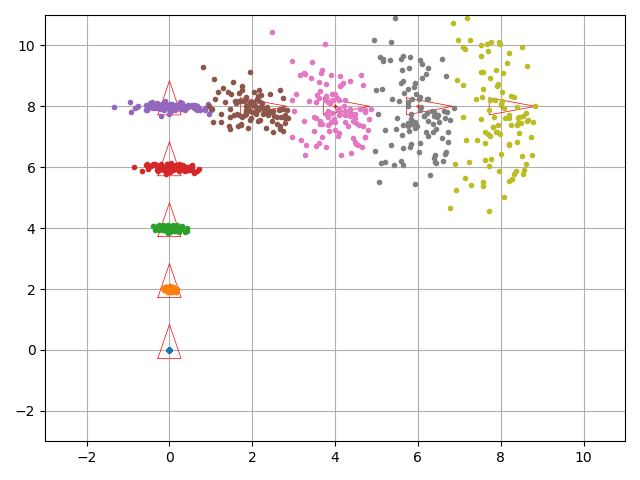
\includegraphics{returns/332.PNG}
\end{figure}    

    \hypertarget{thinking-about-it-2}{%
\subsubsection{Thinking about it (2)}\label{thinking-about-it-2}}

Now you are an expert in the sample form of the odometry motion model!
\textbf{Answer the following questions}:

\begin{itemize}
\item
  Which is the effect of modifying the robot's intrinsic noise
  \(\alpha\) (\texttt{a} in the code)?

  As more as we increase \texttt{a} value, more dispersed will the
  values be
\item
  How many parameters compound the motion command \(u_t\) in this model?

  Three. Angle towards the destiny point, distance to destiny point and
  the desired angle
\item
  After moving the robot a sufficient number of times, what shape does
  the distribution of samples take?

  It have a shape of a half ellipse
\end{itemize}


    % Add a bibliography block to the postdoc
    
    
    
\end{document}
